\documentclass[12pt]{article}

\usepackage[margin=1.1in]{geometry}
\usepackage{amsmath,amssymb,amsthm}
\usepackage{booktabs}
\usepackage{graphicx}
\usepackage[numbers,square,sort&compress]{natbib}
\usepackage[colorlinks=true,citecolor=blue,linkcolor=blue,urlcolor=blue]{hyperref}
\usepackage{microtype}
\usepackage{enumitem}

\newtheorem{theorem}{Theorem}
\newtheorem{proposition}{Proposition}
\newtheorem{lemma}{Lemma}
\newtheorem{corollary}{Corollary}
\theoremstyle{definition}
\newtheorem{definition}{Definition}
\newtheorem{assumption}{Assumption}
\theoremstyle{remark}
\newtheorem{remark}{Remark}

\newcommand{\E}{\mathbb{E}}
\newcommand{\Prob}{\mathbb{P}}
\newcommand{\Var}{\mathrm{Var}}
\newcommand{\ov}{\mathrm{ov}}
\newcommand{\M}{\mathcal{M}}
\newcommand{\TV}{\mathrm{TV}}
\newcommand{\sgm}{\mathrm{sig}}
\DeclareMathOperator*{\essinf}{ess\,inf}
\setlength{\emergencystretch}{3em}

% generated by make_separation_tables.py; do not edit
% result commits: 5666bf203822980171b06bd8da9fa46a0ca2df69
\newcommand{\costUniform}{50.0}
\newcommand{\costOptimal}{44.4}
\newcommand{\costCommon}{988.2}
\newcommand{\costCommonTau}{0.110}
\newcommand{\costRatioCommonUniform}{19.8}
\newcommand{\finiteBound}{51.9}
\newcommand{\finiteConstant}{52.4}
\newcommand{\finiteSlope}{0.808}
\newcommand{\mixtureCost}{46.36}
\newcommand{\covFiveK}{0.9458}
\newcommand{\covFiveKmcse}{0.0032}
\newcommand{\covFiveKseRatio}{0.993}
\newcommand{\covSmallNtau}{0.887}
\newcommand{\smallNtau}{10}

% generated by make_separation_tables.py; do not edit
\newcommand{\tabDesigns}{%
\begin{tabular}{llrrrrr}
\toprule
$\delta$ & design & RMSE & coverage & MCSE & explored & loss $R_n$ \\
\midrule
0.10 & uniform mixing & 0.098 & 0.950 & 0.011 & 100 & 49.9 \\
0.10 & $p\propto g^{-1/2}$ (= context temp.) & 0.103 & 0.932 & 0.013 & 134 & 44.5 \\
0.10 & common temperature & 0.097 & 0.965 & 0.009 & 7607 & 988.5 \\
0.05 & uniform mixing & 0.052 & 0.955 & 0.010 & 400 & 200.3 \\
0.05 & $p\propto g^{-1/2}$ (= context temp.) & 0.053 & 0.940 & 0.012 & 532 & 178.0 \\
0.05 & common temperature & 0.050 & 0.948 & 0.011 & 9191 & 1440.1 \\
\bottomrule
\end{tabular}}
\newcommand{\tabBoundary}{%
\begin{tabular}{rrrrrrrr}
\toprule
$\zeta$ & $n$ & $n\tau_n$ & reps & RMSE & coverage of $\beta_0$ & MCSE & loss $R_n$ (theory) \\
\midrule
0.60 & 10{,}000 & 39.8 & 1{,}000 & 0.215 & 0.949 & 0.007 & 0.1290 (0.1304) \\
0.60 & 100{,}000 & 100.0 & 500 & 0.141 & 0.944 & 0.010 & 0.0821 (0.0822) \\
0.60 & 1{,}000{,}000 & 251.2 & 200 & 0.082 & 0.970 & 0.012 & 0.0513 (0.0519) \\
0.75 & 10{,}000 & 10.0 & 1{,}000 & 0.464 & 0.887 & 0.010 & 0.0081 (0.0082) \\
0.75 & 100{,}000 & 17.8 & 500 & 0.339 & 0.924 & 0.012 & 0.0026 (0.0026) \\
0.75 & 1{,}000{,}000 & 31.6 & 200 & 0.247 & 0.930 & 0.018 & 0.0008 (0.0008) \\
0.60 & 1{,}000{,}000 & 251.2 & 5{,}000 & -- & 0.946 & 0.003 & -- \\
\bottomrule
\end{tabular}}


\title{The exploration cost of boundary and population effects}
\author{Kunwoo Park\thanks{\textbf{[TO CONFIRM: department]}, Kookmin University,
Seoul, Republic of Korea. Corresponding author. E-mail: \textbf{[TO CONFIRM]}.}}
\date{}

\begin{document}
\maketitle

\begin{abstract}
\noindent Can a growing deployment support causal inference while the operational
cost of experimentation vanishes? The answer depends on the effect being
estimated. We study known assignment policies that increasingly favor a
preferred action and measure exploration by the cumulative operational value
forgone through alternative actions. In one model with a one-dimensional
score and mean outcomes that are Lipschitz near the decision boundary, a
shrinking common temperature permits pointwise asymptotically valid inference
for the boundary effect while exploration loss tends to zero. The same model
contains outcome laws with identical boundary effects but different population
average effects that become indistinguishable under vanishing loss. Uniform
mean-square consistency for the population effect requires divergent
worst-case loss. In a larger model without extrapolation restrictions, an
information--exploration inequality applies to all estimators and adaptive
designs, with a lower-bound constant involving the operational gap functional
$(\E\sqrt g)^2$. For sufficiently small fixed target error, one deterministic
common temperature requires loss growing at least as $n/\log^2 n$, while
uniform mixing has bounded loss. Conversational AI motivates the setting;
the formal results concern a single strategy assignment per independent unit,
with the text-generation kernel held fixed.
\end{abstract}

\noindent\textbf{Keywords:} adaptive experiments, limited overlap, regression
discontinuity, exploration, generative AI, off-policy evaluation

\noindent\textbf{MSC 2020:} 62D20, 62K05, 62C20, 62G20

%=============================================================================
\section{Introduction}\label{sec:intro}

A deployment can generate increasingly many observations while providing
very different information about different causal effects. Under a shrinking common temperature, alternative actions become
concentrated near the decision boundary. Those comparisons can support local
inference at a decreasing operational cost. Learning an average effect over
all contexts requires comparisons elsewhere as well. This paper quantifies
that difference using one outcome model and one exploration-loss criterion.

Conversational artificial intelligence provides a motivating example. In randomized trials, GPT-4
shifted debate opponents' positions more often than human debaters did
\cite{salvi2025conversational}, and conversations with frontier models moved
policy attitudes with effects that persisted for weeks
\cite{hackenburg2025levers}. Establishing that a technology persuades is the
first question, not the last. Regulation and replication concern narrower
objects: whether presenting evidence rather than asking a question, at this
point in this conversation, changes what a person believes. Systems that
persuade at scale choose such strategies adaptively, and their logs are what
an analyst inherits. One of the strongest levers identified by
Hackenburg et al.~\cite{hackenburg2025levers}, a reward model that selects among candidate
responses, is itself an adaptive selection policy.

This paper asks a precise version of the question those logs raise. Suppose
the deployer's strategy policy is known, as it is when the deployer records
action probabilities, and suppose it sharpens as the deployer becomes
confident, for instance by lowering a softmax temperature. Which causal
effects can the logs estimate, and what must be paid to estimate the others?

The answer depends on the target. We distinguish two:
\begin{itemize}[leftmargin=1.5em,itemsep=2pt]
\item the \emph{boundary effect}, the effect among contexts where the policy is
indifferent between strategies; and
\item the \emph{population average effect} over all contexts the deployment
serves.
\end{itemize}
These answer different questions. The first is relevant to marginal changes
of a policy that is already deployed; the second to the average outcome change from assigning strategy $1$
rather than strategy $0$ across the full context population, holding the
generator fixed. Estimating one well does not substitute for estimating the
other.

We price learning in the deployer's own currency. Each time the logged
strategy differs from the one the deployer's objective prefers, the deployer
gives up an operational value gap $g(h)$. The cumulative sum is the
\emph{exploration loss} $R_n$. This quantity is defined by the deployer's
objective, not by the human outcome under study, so it can be computed at the
design stage without knowing the effects being estimated.

Figure~\ref{fig:separation} previews the construction behind
Theorem~\ref{thm:separation}. Perturbing only the
unpreferred action away from the boundary changes the population effect but
leaves the boundary effect unchanged. A sharpening policy produces very few
observations of precisely that action in the perturbed region.

\begin{figure}[htbp]
\centering
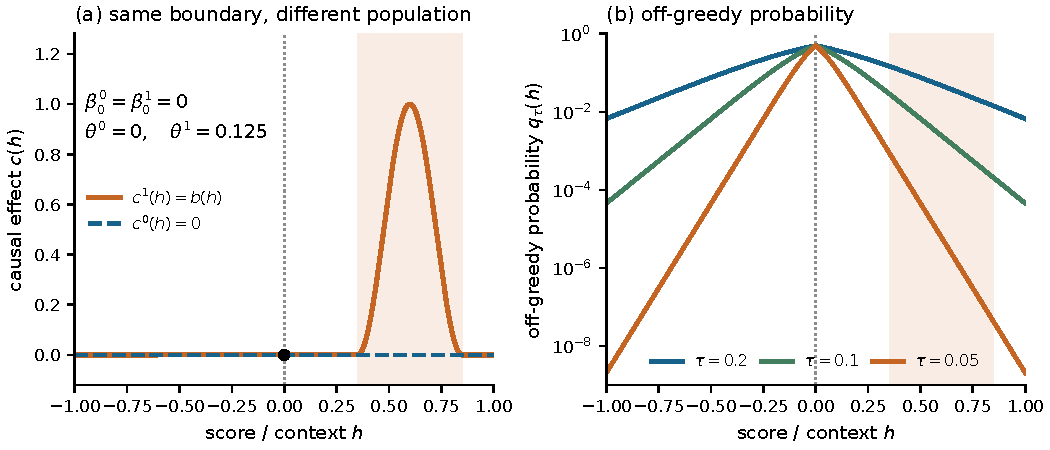
\includegraphics[width=\textwidth]{figs/fig1_mechanism.pdf}
\caption{The separation construction, with $H\sim U(-1,1)$, $g(h)=|h|$,
$u_1=0.35$, $u_2=0.85$, and $t=1$. Left: the two effect functions $c^0=0$
and $c^1=b$ (superscripts index outcome laws) have the same boundary effect,
zero, but population effects $0$
and $0.125$. The greedy-arm mean is unchanged. Right: the probability of an
off-greedy action under three illustrative temperatures. Shading marks the
region in which the outcome laws differ. These are exact functions from the
construction, not simulation estimates or fitted effects.}
\label{fig:separation}
\end{figure}

\paragraph{Contributions.}
\begin{enumerate}[leftmargin=1.5em,itemsep=3pt]
\item \emph{Separation in one model} (Theorem~\ref{thm:separation}). In a
one-dimensional score model with Lipschitz mean outcomes near the decision
boundary, logs generated by a single common temperature
$\tau_n = n^{-\zeta}$, $\zeta\in(1/2,1)$, give asymptotically valid Wald
intervals for the boundary effect at every member of the model, while
$R_n\to0$ (Theorem~\ref{thm:boundary}). In the same model, whenever $R_n\to0$,
two members that coincide near the boundary but differ in the population
effect have total variation distance tending to zero, so no estimator is
consistent for the population effect at both; and uniform consistency for the
population effect requires $\sup R_n\to\infty$. Figure~\ref{fig:map} shows the
separation in exact risks for a simple design.
\item \emph{An information--exploration inequality}
(Theorem~\ref{thm:info}). In the model of all bounded mean functions, for
every estimator and every adaptive or non-adaptive design, the product of
worst-case mean squared error and worst-case exploration loss plus a constant
is at least $\sigma^2(\sum_k f_k\sqrt{g_k})^{2}$. Uniform precision $\delta$
therefore requires worst-case exploration loss at least of order
$(\E\sqrt g)^2/\delta^2$ as the target error tends to zero; a design exploring with
probability proportional to $g^{-1/2}$ attains this order up to constants
(Proposition~\ref{prop:achieve}).
\item \emph{What this means for temperature.} For any sufficiently small fixed
precision $\delta$, a single deterministic common temperature requires
exploration loss at least of order $n/\log^2(n\delta^2)$
(Theorem~\ref{thm:common}), against a loss of order $\delta^{-2}$, bounded in
$n$, for the designs below. Context-dependent temperatures implement the
gap-based design (Proposition~\ref{prop:ctx}). Random mixtures of finite temperatures can also
avoid the rate (Remark~\ref{rem:mixture}). When the value gap is misspecified,
a Kantorovich bound says when gap-based allocation is worth its risk relative
to uniform mixing (Lemma~\ref{lem:robust}).
\end{enumerate}

\paragraph{Scope.} All results are for one decision per unit with independent
contexts and a known assignment policy. Theorem~\ref{thm:boundary} and
Theorem~\ref{thm:separation} use a one-dimensional score, and their boundary
guarantees are pointwise in the outcome law. The impossibility results hold
in models without extrapolation structure: where data near the boundary
identify the population effect, as under a constant effect, the separation
disappears. Multi-turn conversations, estimated policies, and effects of
realized text features are outside the formal results.

\paragraph{Relation to existing work.}
\emph{Boundary estimands from algorithmic assignment.}
Narita and Yata~\cite{narita2021algorithm} show that weights of overlap type, built from an
approximate propensity score of a known algorithm, converge to a boundary
estimand and require undersmoothing; this is the closest antecedent for
Theorem~\ref{thm:boundary}. There the smoothing is an analyst-chosen ball in
covariate space; here it is a temperature chosen by the system in score space,
and we compute the exploration loss jointly with the inferential guarantee.
Eckles et al.~\cite{eckles2020noise} use known assignment noise near a cutoff for
design-based inference, with a fixed noise scale and no cost accounting.
Overlap weights and their target population are due to
Li, Morgan and Zaslavsky~\cite{li2018balancing}; they note that the weights peak where the propensity
score is one half, but do not study a sharpening limit. Humphreys~\cite{humphreys2025bounds}
shows that the fixed-effects estimand weights stratum effects by the assignment
variance $p_j(1-p_j)$, the same weighting, and can differ from the average
effect; under a sharpening policy this weighting concentrates on the decision
boundary.

\emph{Exploration and estimation.} Simchi-Levi and Wang~\cite{simchilevi2023multi} show a
regret--estimation trade-off in multi-armed bandits without contexts;
Wan, Kveton and Song~\cite{wan2022safe} optimize exploration for policy evaluation under a value
constraint; Douglas, Persson and Provost~\cite{douglas2026logging} derive optimal logging policies for
inverse-propensity estimation and report that softmax logging performs worse
than top-$k$ logging in simulation; Koppel et al.~\cite{koppel2025explore} extend
inverse-gap-weighting contextual bandits to balance regret against the quality
of average-treatment-effect estimates (we have read only the abstract of that
workshop paper). The allocation $q\propto g^{-1/2}$ has the
form of optimum stratified allocation with costs \cite{cochran1977sampling},
and Ravichandran et al.~\cite{ravichandran2024optimal} derive the analogous
cost-weighted rule, sample sizes proportional to $S_j/\sqrt{C_j}$, for factorial
experiments under a budget. We do not claim the allocation as new; what we add
is that the corresponding constant bounds every estimator and adaptive design
when loss is paid only for off-greedy actions. Li and
Imai~\cite{li2024neyman} compare evaluating an individualized treatment rule by
randomizing units to the rule with evaluation from a standard experiment,
without a cost for assignments against the rule; our exploration loss makes
that cost explicit. Cesa-Bianchi et al.~\cite{cesabianchi2017boltzmann} show
that Boltzmann exploration with a common schedule can fail for regret and that
arm-dependent schedules repair it; our Theorem~\ref{thm:common} and
Proposition~\ref{prop:ctx} are estimation analogues.

\emph{Limited overlap and off-policy evaluation.} Lower bounds for
off-policy value estimation \cite{li2015toward,wang2017optimal,mou2023off}
and limited-overlap asymptotics
\cite{khan2010irregular,hong2020inference,ma2020robust} supply the
information-theoretic ingredients. Khan and Tamer~\cite{khan2010irregular} observe that the
average treatment effect loses identification when any region of the
covariate support is removed, and derive rates for trimmed inverse weighting
when propensities approach zero or one in the covariate tails; their
propensities do not change with $n$, and there is no cost of exploration.
What we add is the coupling of the
information bound to the exploration loss, and the comparison of boundary and
population targets on that common scale. Ring and
Schomaker~\cite{ring2026diagnostic} give a diagnostic for stochastic positivity
problems and use it to choose alternative estimands when the data do not
support the original one; our results are a formal counterpart for known,
sharpening assignment policies, stating which estimand remains learnable and at
what exploration cost. Khan, Saveski and Ugander~\cite{khan2024off} bound effects
without overlap under smoothness, which is the kind of extrapolation structure
our impossibility excludes.

\emph{Generative treatments.} Athey, Imbens and Ji~\cite{athey2026stochastic} identify effects of
content features from stochastic algorithms using logged unexposed candidates
and probability ratios. Their estimand averages over co-occurring pairs with
trimming and does not conflict with our bounds, which concern the population
effect of a strategy under outcomes observed only for the logged action.
Fresh and Shin~\cite{fresh2026conversation} give a taxonomy of conversational estimands;
we work at the level of strategy assignment. Imai and Nakamura~\cite{imai2026causal} and
Nakamura and Imai~\cite{nakamura2026dynamic} study effects of realized text features under
deterministic decoding; we instead hold the generation kernel fixed.

%=============================================================================
\section{Setup}\label{sec:setup}

\paragraph{Generative treatments.} Units $i=1,\dots,n$ arrive with contexts
$H_i\sim F$, independently. The system chooses a strategy $A_i\in\{0,1\}$ and
produces a message $M_i\sim G(\cdot\mid A_i,H_i)$ from a fixed generation
kernel $G$, which includes token-level sampling settings. The outcome is
$Y_i$. The treatment is assignment of the strategy with $G$ held fixed:
potential outcomes $Y_i(a)$ are defined under the kernel intervention that
sets $A_i=a$ and draws the message from $G$
\cite{munoz2012population,young2014identification}. A label attached to a
realized message after the fact is a different object, and changing $G$, for
example by changing token temperature, changes the treatment. We assume:
\begin{enumerate}[label=(C\arabic*),leftmargin=3em,itemsep=1pt]
\item \emph{consistency}: $Y_i=Y_i(A_i)$, where the randomness of the message
drawn from $G$ is part of $Y_i(a)$;
\item \emph{independent units}: $(H_i,Y_i(0),Y_i(1))$ are independent and
identically distributed across $i$, with no interference;
\item \emph{known sequential assignment}: given $H_i$ and the past data
$\mathcal F_{i-1}$, $A_i$ is drawn with known probabilities, independently of
$(Y_i(0),Y_i(1))$ and of all future units.
\end{enumerate}
Under (C1)--(C3),
$\E[Y_i\mid A_i=a,H_i=h,\mathcal F_{i-1}]=\E[Y(a)\mid H=h]$, and the law of
$Y_i$ given $(A_i=a,H_i=h,\mathcal F_{i-1})$ is that of $Y(a)$ given $H=h$.
All statements below about conditional outcome laws are therefore statements
about potential outcomes.

\paragraph{Deployer.} The deployer has a score gap $\Delta(h)=s_1(h)-s_0(h)$
from its own objective, a greedy strategy $a^*(h)=\mathbf 1\{\Delta(h)>0\}$,
and an operational value gap $g(h)\ge0$, the value its objective loses by
choosing $\bar a(h)=1-a^*(h)$. We write $g=\phi(|\Delta|)$ when the gap is a
function of the score.

\paragraph{Designs and notation for probabilities.} We use two probabilities
and keep them distinct:
\[
e(h)=\Prob(A=1\mid H=h),\qquad q(h)=\Prob(A\neq a^*(h)\mid H=h),
\]
the probability of strategy $1$ and the probability of the off-greedy
strategy. A design specifies $Q_i=\Prob(A_i=\bar a(H_i)\mid H_i,\mathcal
F_{i-1})$; it is non-adaptive if $Q_i=q(H_i)$. A \emph{common temperature}
design uses one deterministic $\tau=\tau_n$ and
\[
e_\tau(h)=\sgm(\Delta(h)/\tau),\qquad q_\tau(h)=\sgm(-|\Delta(h)|/\tau),
\]
where $\sgm(x)=1/(1+\exp(-x))$.

\paragraph{Exploration loss.}
We measure expected cumulative operational loss, rather than loss per unit:
\begin{equation}\label{eq:loss-definition}
 R_n=\E\left[\sum_{i=1}^n g(H_i)\mathbf 1\{A_i=\bar a(H_i)\}\right].
\end{equation}
For a non-adaptive design, $R_n=n\E[g(H)q(H)]$. The context law $F$, the score
$\Delta$, and the operational gap $g$ are fixed when comparing outcome laws;
under an adaptive design, $R_n$ can nevertheless depend on the outcome law
through past observations.

\paragraph{Estimands.} Let $\mu_a(h)=\E[Y(a)\mid H=h]$ and $c=\mu_1-\mu_0$.
The population average effect is $\theta=\E[c(H)]$. With a one-dimensional
score $\Delta(h)=h$, the boundary effect is $\beta_0=c(0)$. For a given
temperature, the overlap-weighted effect
$\beta_{\ov,\tau}=\E[\omega_\tau(H)c(H)]/\E[\omega_\tau(H)]$ with
$\omega_\tau=e_\tau(1-e_\tau)$ \cite{li2018balancing} is a third,
temperature-indexed, target; we use it only as an intermediate object.

%=============================================================================
\section{Boundary effects at vanishing exploration loss}\label{sec:boundary}

\begin{assumption}[Boundary model]\label{ass:D}
$\Delta(h)=h$, $a^*(h)=\mathbf 1\{h>0\}$, and
\begin{enumerate}[label=(D\arabic*),leftmargin=3em,itemsep=1pt]
\item $H$ has a density $f\le\bar f$, continuous at $0$, with $f(0)>0$;
\item $|\mu_a|\le B$, and $\mu_a$ is $L$-Lipschitz on $[-u_0,u_0]$;
\item $\sigma_a^2(h)=\Var(Y\mid A=a,H=h)$ is continuous at $0$ with
$\sigma_1^2(0)+\sigma_0^2(0)>0$, and $\E[Y^4\mid A,H]\le M$;
\item $\Prob(A=1\mid H=h)=\sgm(h/\tau_n)$ with $\tau_n\to0$, known;
\item $g=\phi(|h|)\le\bar G$ with $\phi(u)\le\bar\kappa u$ on $[0,u_0]$; in the
strong form $\phi'(0)=\kappa>0$.
\end{enumerate}
\end{assumption}

With $e_i=e_{\tau_n}(H_i)$, define the overlap weights and arm means by
\begin{align}
 w_{1i}&=A_i(1-e_i), & w_{0i}&=(1-A_i)e_i,\nonumber\\
 \hat D_a&=\frac1n\sum_{i=1}^n w_{ai}, &
 \hat m_a&=\frac{\sum_{i=1}^n w_{ai}Y_i}{\sum_{i=1}^n w_{ai}},
 &\hat\beta&=\hat m_1-\hat m_0.\label{eq:boundary-estimator}
\end{align}
For inference use
\begin{align}
 \hat\psi_i&=\frac{w_{1i}(Y_i-\hat m_1)}{\hat D_1}
             -\frac{w_{0i}(Y_i-\hat m_0)}{\hat D_0},\nonumber\\
 \hat s^2&=\frac1n\sum_{i=1}^n\hat\psi_i^2,
 &\widehat{\mathrm{SE}}(\hat\beta)&=\frac{\hat s}{\sqrt n}.
 \label{eq:boundary-se}
\end{align}
If either denominator is zero, set $\hat m_a$, $\hat\beta$, $\hat s^2$
and the undefined influence values to zero, and report the interval
$\mathbb R$. This event has probability tending to zero under the theorem's
conditions; it does not change the asymptotic conclusions.

\begin{theorem}[Boundary inference]\label{thm:boundary}
Under Assumption~\ref{ass:D}, if $n\tau_n\to\infty$:
\begin{enumerate}[label=(\roman*),leftmargin=2em,itemsep=1pt]
\item $(\hat\beta-\beta_{\ov,\tau_n})/(s_n/\sqrt n)\Rightarrow N(0,1)$ with
$s_n^2=\{\sigma_1^2(0)+\sigma_0^2(0)\}/\{2\tau_nf(0)\}\,(1+o(1))$;
\item $|\beta_{\ov,\tau_n}-\beta_0|\le C\tau_n$ for large $n$;
\item $\hat s^2/s_n^2\to1$ in probability;
\item if also $n\tau_n^3\to0$, the Wald interval $\hat\beta\pm
z_{1-\eta/2}\hat s/\sqrt n$ has asymptotic coverage $1-\eta$ for $\beta_0$;
\item $R_n=n\E[g(H)q_{\tau_n}(H)]\le n\tau_n^2\bar\kappa\bar f\pi^2/6+n\bar G\exp(-u_0/\tau_n)$, and in
the strong form $R_n=n\tau_n^2\kappa f(0)\pi^2/6\,(1+o(1))$.
\end{enumerate}
In particular, for $\tau_n=n^{-\zeta}$ with $\zeta\in(1/2,1)$, the interval in
(iv) is asymptotically valid and $R_n\to0$.
\end{theorem}

The three rate conditions are $n\tau_n\to\infty$ (the boundary sample grows,
$\zeta<1$), $n\tau_n^3\to0$ (bias is negligible relative to the standard
error, $\zeta>1/3$), and $n\tau_n^2\to0$ (the loss vanishes, $\zeta>1/2$). The
error $|\hat\beta-\beta_0|=O_p((n\tau_n)^{-1/2})$ is achievable; we do not
claim it is optimal, and it is a statement in probability rather than in mean
square. Differentiability of $c$ at zero does not improve the bias order in
general: a bounded effect equal to $c(h)=1+|h|^{3/2}$ near zero
gives bias proportional to $\tau^{3/2}$. If $c$ is
$C^{1,1}$ and $f$ is Lipschitz near zero, the bias is $O(\tau^2)$ and
condition (iv) relaxes to $n\tau_n^5\to0$. Proofs are in
Appendix~\ref{app:boundary}.

Vanishing loss does not mean that exploration disappears. The expected number
of off-greedy actions is $n\E[q_{\tau_n}(H)]=2\log2\,f(0)\,n\tau_n(1+o(1))$,
which grows because $n\tau_n\to\infty$; the loss nevertheless vanishes,
$R_n=O(n\tau_n^2)$, with asymptotic equivalence in the strong form of
(D5), because these actions occur ever closer to the boundary,
where the value gap is small.

%=============================================================================
\section{Population effects require paid exploration}\label{sec:population}

Fix $B>0$ and $\sigma>0$. Let $\M(B,\sigma)$ be the model in which $Y\mid A=a,H=h$ is $N(\mu_a(h),\sigma^2)$
and $\mu_0,\mu_1$ are \emph{any} measurable functions bounded by $B$. The
model contains no structure that carries effects learned near the boundary to
other contexts.

\begin{theorem}[Information--exploration inequality]\label{thm:info}
Let $S_1,\dots,S_K$ be disjoint sets with $f_k=F(S_k)>0$, each contained in
$\{a^*=0\}$ or in $\{a^*=1\}$, and $g_k=\inf_{S_k}g$. For every design,
adaptive or not, and every estimator $\hat\theta$,
\begin{equation}\label{eq:info}
\sup_{\M(B,\sigma)}\E(\hat\theta-\theta)^2\cdot
\Big(\sup_{\M(B,\sigma)}R_n+\frac{\sigma^2\pi^2}{B^2}\sum_k g_k\Big)
\;\ge\;\sigma^2\Big(\sum_kf_k\sqrt{g_k}\Big)^2 .
\end{equation}
Consequently, if $F(g\ge\gamma)>0$ for some $\gamma>0$, uniform consistency
requires $\sup R_n\to\infty$; and if $\sup\E(\hat\theta-\theta)^2\le\delta_n^2\to0$,
then $\liminf_n\delta_n^2\sup R_n\ge\sigma^2(\E\sqrt{g(H)})^2$.
\end{theorem}

Neither side of \eqref{eq:info} involves $n$: deployment scale does not
substitute for exploration when the target is the population effect. If
$\sum_k g_k>0$, at $R_n=0$ the bound is the finite floor
$B^2(\sum f_k\sqrt{g_k})^2/(\pi^2\sum g_k)$, consistent with the fact that a
constant estimator has bounded error.

\begin{proposition}[Achievability]\label{prop:achieve}
Suppose $0<\E\sqrt g<\infty$, $\delta_n>0$, and $n\delta_n^2\to\infty$. Write
$C=\sigma^2+B^2$. For $n\delta_n^2>4C$, define
\begin{equation}\label{eq:allocation}
 c_n=\frac{\E\sqrt g}{n\delta_n^2/C-4},\qquad
 q_n(h)=\begin{cases}
 \min\{1/2,c_n/\sqrt{g(h)}\},&g(h)>0,\\
 1/2,&g(h)=0.
 \end{cases}
\end{equation}
Let $e_n(h)$ be the corresponding probability of strategy $1$. Then
\begin{equation}\label{eq:ht}
 \hat\theta_{\rm HT}=\frac1n\sum_{i=1}^n
 \left\{\frac{A_iY_i}{e_n(H_i)}-
 \frac{(1-A_i)Y_i}{1-e_n(H_i)}\right\}
\end{equation}
has $\sup_{\M(B,\sigma)}\E(\hat\theta_{\rm HT}-\theta)^2\le\delta_n^2$, and
\[
 R_n\le\frac{Cn(\E\sqrt g)^2}{n\delta_n^2-4C}
      =C(\E\sqrt g)^2\delta_n^{-2}(1+o(1)).
\]
If also $\E[g]<\infty$, uniform mixing with
$q\equiv C/(n\delta_n^2-2C)$, for $n\delta_n^2\ge4C$, has the same uniform
risk guarantee and
\[
 R_n=\frac{Cn\E[g]}{n\delta_n^2-2C}
    =C\E[g]\delta_n^{-2}(1+o(1)).
\]
\end{proposition}

The order $\delta^{-2}$ and the functional $(\E\sqrt g)^2$ therefore appear in
both the lower bound and the attainable loss. These upper bounds are constructive guarantees;
they do not assert exact finite-sample optimality of the allocation.
The constants differ: the lower
bound has $\sigma^2$, and the Horvitz--Thompson upper bound retains $B^2$. We
do not establish the optimal constant. Proofs are in Appendix~\ref{app:population}.

%=============================================================================
\section{The separation}\label{sec:separation}

Theorem~\ref{thm:info} is proved in $\M(B,\sigma)$, while
Theorem~\ref{thm:boundary} assumes Lipschitz means near the boundary. A lower
bound over a large model does not transfer to a smaller one automatically. We
therefore state both sides in one model.

Let $\M_D$ be the set of outcome laws satisfying (D1), (D2), Gaussian noise
with variance $\sigma^2$, and (D5) with $\phi$ not necessarily monotone. Under
Gaussian noise, (D3) holds for every member of $\M_D$.

\begin{assumption}\label{ass:SA}
There are $u_0<u_1<u_2$ with $F([u_1,u_2])>0$ and
$\gamma:=\essinf_{h\in[u_1,u_2]}g(h)>0$, and $B,L>0$.
\end{assumption}

\begin{theorem}[Separation]\label{thm:separation}
Under Assumption~\ref{ass:SA}, let
$b(h)=\sin^2(\pi(h-u_1)/(u_2-u_1))\mathbf 1\{u_1\le h\le u_2\}$,
$t_{\max}=\min\{B,L(u_2-u_1)/\pi\}$, and for $|t|\le t_{\max}$ let $\mu^t\in\M_D$
have $\mu^t_1\equiv0$ and $\mu^t_0=-tb$. All $\mu^t$ coincide on
$(-\infty,u_1]$, have boundary effect $\beta_0=0$, and have population effect
$\theta(\mu^t)=t\E[b(H)]$.
\begin{enumerate}[label=(S\arabic*),leftmargin=3em,itemsep=2pt]
\item Under the common-temperature design $\tau_n=n^{-\zeta}$,
$\zeta\in(1/2,1)$, $R_n\to0$ and, for every $\mu\in\M_D$, the Wald interval of
Theorem~\ref{thm:boundary} has asymptotic coverage $1-\eta$ for $\beta_0(\mu)$.
\item For every design and every $t$,
$\TV(P^n_{\mu^0},P^n_{\mu^t})\le R_n(\mu^0)/\gamma$. Hence if
$R_n(\mu^0)\to0$, for every $t_1\in(0,t_{\max}]$ and every estimator,
$\max_{t\in\{0,t_1\}}P_{\mu^t}(|\hat\theta_n-\theta(\mu^t)|\ge t_1\E[b]/2)\ge
(1-R_n(\mu^0)/\gamma)/2\to1/2$.
\item For every design and every estimator,
\[
\sup_{\M_D}\E(\hat\theta-\theta)^2\ge\frac{(\E[b])^2}{\sup_{\M_D}R_n/(\sigma^2\gamma)+\pi^2/t_{\max}^2}.
\]
\end{enumerate}
\end{theorem}

Under the design of (S1), $\mu^0$ and $\mu^{t_1}$ are both members of $\M_D$
with the same boundary effect, and the boundary interval is valid at each.
By (S2), no estimator of the population effect is consistent at both. By
(S3), consistency uniformly over $\M_D$ requires unbounded exploration loss.
We do not claim that the constant of Theorem~\ref{thm:info} holds in
$\M_D$, nor any uniform guarantee on the boundary side. If a submodel lets
boundary data identify $\theta$, the perturbation family is excluded and
(S2)--(S3) do not apply. Proofs are in Appendix~\ref{app:separation}.

Figure~\ref{fig:map} illustrates the separation with exact risks, computed by
numerical integration, for the design used in Section~\ref{sec:sims}. Under one
common temperature, the population effect reaches root mean squared error
$\figDelta$ only where the exploration loss is large: on the plotted grid the
smallest such loss is about $\figPopMinLoss$. The boundary effect reaches the
same precision with loss $\figBndMinLoss$ at the edge of the grid, and with less
loss at larger $n$ and sharper policies.

\begin{figure}[htbp]
\centering
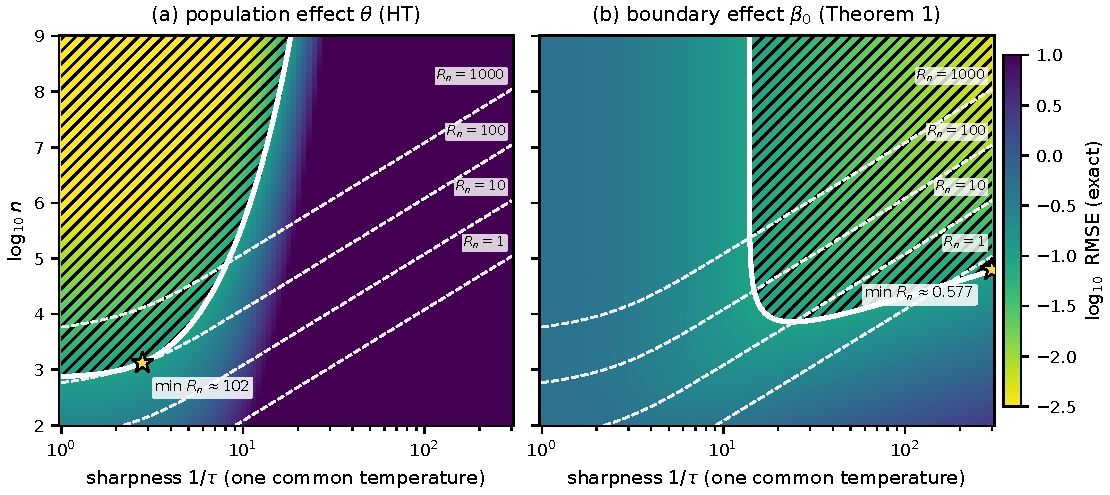
\includegraphics[width=\textwidth]{figs/fig2_separation_map.pdf}
\caption{Exact root mean squared error (colour, $\log_{10}$ scale) under one
common temperature $\tau$ for the design of Section~\ref{sec:sims}: $H\sim
U(-1,1)$, $\Delta(h)=h$, $g(h)=|h|$, $c(h)=1+|h|$, unit noise. (a) The
Horvitz--Thompson estimator of the population effect $\theta$. (b) The
estimator of Theorem~\ref{thm:boundary} for the boundary effect $\beta_0$,
including its bias. Hatched regions, bounded by white curves, have root mean
squared error at most $\figDelta$. Dashed curves are levels of the cumulative
exploration loss $R_n=n\E[g(H)q_\tau(H)]$. Stars mark the smallest loss that
attains the precision on the plotted grid ($1\le1/\tau\le300$,
$10^2\le n\le10^9$). Panel (a) concerns one estimator under one outcome law; the
lower bounds for all estimators are Theorems~\ref{thm:info}
and~\ref{thm:separation}.}
\label{fig:map}
\end{figure}

%=============================================================================
\section{Temperature as an exploration device}\label{sec:temperature}

\begin{theorem}[One common temperature]\label{thm:common}
Consider common-temperature designs with one deterministic $\tau_n$ per $n$.
Assume $g=\phi(|\Delta|)$, $\E[g]<\infty$, and $|\Delta(H)|$ has a density at least $f_{\min}>0$ on $[0,u_0]$;
$\phi(u)\ge\kappa u$ on $[0,u_0]$; $D_{\max}=\operatorname{ess\,sup}|\Delta(H)|<\infty$;
and for every $\eta'\in(0,D_{\max})$, $\nu_{\eta'}=\max_j\Prob(|\Delta(H)|\ge
D_{\max}-\eta',a^*(H)=j)>0$. Fix $\eta'\in(0,D_{\max})$. If an estimator has
$\sup_{\M(B,\sigma)}\E(\hat\theta-\theta)^2\le\delta_n^2$ with
$\delta_n^2\le\nu_{\eta'}^2B^2/(2\pi^2)$ and $2n\delta_n^2>\nu_{\eta'}\sigma^2$,
then
\[
R_n\ \ge\ \kappa f_{\min}c_0\,n\min\Big\{u_0^2,\ \frac{(D_{\max}-\eta')^2}{\log^2\{2n\delta_n^2/(\nu_{\eta'}\sigma^2)\}}\Big\},
\qquad c_0=\int_0^1v\,\sgm(-v)\,dv .
\]
\end{theorem}

This is a lower bound, and $\delta_n$ may be fixed. For any fixed $\delta$ with
$\delta^2\le\nu_{\eta'}^2B^2/(2\pi^2)$, the common-temperature loss is at least of
order $n/\log^2 n$, whereas Proposition~\ref{prop:achieve} attains the same
uniform precision with loss bounded in $n$. The precision condition cannot be
dropped: for $\delta\ge2B$ the estimator that always outputs zero meets the
target with no exploration. Relative to the attainable loss, the lower bound is
larger by a factor of order at least $n\delta_n^2/\log^2(n\delta_n^2)$, which
diverges whenever $n\delta_n^2\to\infty$. With finitely many score values
$0<\Delta_{\min}<\Delta_{\max}$ and fixed, sufficiently small $\delta$, the
common-temperature loss is at least of order $n^{1-\Delta_{\min}/\Delta_{\max}}$. The reason is not that a
common temperature explores in the wrong place: the optimal design also
explores most near the boundary, where the operational gap is small. It is that the
exploration probability of a common temperature decays exponentially in
$|\Delta|$, so observations far from the boundary become too rare unless the
temperature is raised everywhere, which is expensive near the boundary.

\begin{remark}[Mixtures of temperatures]\label{rem:mixture}
Theorem~\ref{thm:common} does not extend to random mixtures of finite
temperatures. With $|\Delta|=|H|$, $H\sim U(-1,1)$, $g=|H|$, mixing
temperature $1$ with weight $w_n=\E[1/\sgm(-|H|)]/(n\delta^2)$ and temperature
$1/n$ otherwise keeps the design variance $\E[1/q]/n$ at most $\delta^2$, for
fixed $\delta$, with loss bounded in $n$
(\mixtureCost{} at $\delta=0.1$ for $n=10^4,10^5,10^6$). The lesson concerns a
single common temperature, not temperature as such.
\end{remark}

\begin{proposition}[Context temperatures]\label{prop:ctx}
For $\Delta(h)\neq0$ and $q(h)\in(0,1/2)$, the context temperature
$\tau(h)=|\Delta(h)|/\log\{(1-q(h))/q(h)\}$ gives off-greedy probability
$q(h)$. The value $q(h)=1/2$ requires $\tau(h)=\infty$, and on $\{\Delta=0\}$ every
temperature gives $q=1/2$. Suppose $g=\phi(|\Delta|)$ with $\phi(0)=0$, so that
$g=0$ on $\{\Delta=0\}$. Then the design $q^*$ of
Proposition~\ref{prop:achieve} is implementable with temperatures in
$(0,\infty]$: $q^*=1/2$ wherever $g=0$, and for each $h$ with $\Delta(h)\neq0$
and $g(h)>0$, $q^*(h)<1/2$ for large $n$ and $\tau^*(h)\log(1/c_n)\to|\Delta(h)|$.
\end{proposition}

The limit is pointwise for fixed $h$ with $g(h)>0$. It does not say that the
implementing temperature is small near the boundary at finite $n$: where the
cap binds, for example $0<|h|\le4c_n^2$ when $g(h)=|h|$, the implementing
temperature is $\tau=\infty$.

\begin{lemma}[Misspecified gaps]\label{lem:robust}
Assume $F(g>0)=1$, $0<\E\sqrt g<\infty$, and
$0<a\le\hat g/g\le b<\infty$. Compare the designs
$q=c/\sqrt{\hat g}$ and $q=c'/\sqrt g$, with $c,c'$ chosen so that both have
the same sparse-exploration criterion $\sigma^2\E[1/q]/n$, and suppose both
probabilities are at most $1/2$ almost surely. Let $\rho=b/a$. Then the loss ratio is at most
$K(\rho)=(1+\sqrt\rho)^2/(4\sqrt\rho)$. The bound is attained when the measure
$w\propto\sqrt g\,dF$ has a set of mass exactly one half, for example when it
is non-atomic.
\end{lemma}

A common rescaling of $\hat g$ changes nothing; only relative
misspecification across contexts matters. Gap-based allocation beats uniform
mixing for every admissible $\hat g$ if $\E[g]/(\E\sqrt g)^2>K(\rho)$; the
condition is also necessary when the bound is attained, but not in general.
The criterion $\sigma^2\E[1/q]/n$ is not the full estimator MSE.
For capped designs, including gaps with positive probability of being zero,
the ratio bound holds as the inverse-exploration moment tends to infinity. Suppose $0<a\le\hat g/g\le b<\infty$ on $\{g>0\}$, $\hat g=0$ on
$\{g=0\}$, $0<\E\sqrt g<\infty$, and let $q_c=\min\{1/2,c/\sqrt{\hat g}\}$
with $q_c=1/2$ where $\hat g=0$. By dominated convergence,
$c\,\E[1/q_c]=\E\max\{2c,\sqrt{\hat g}\}\to\E\sqrt{\hat g}$ and
$\E[gq_c]/c\to\E[g/\sqrt{\hat g}]$ (with $g/\sqrt{\hat g}=0$ where $g=0$) as
$c\to0$. Calibrating $c$ to a common inverse-exploration moment
$T=\E[1/q_c]\to\infty$,
the loss ratio converges to $\E[\sqrt{\hat g}]\E[g/\sqrt{\hat g}]/(\E\sqrt g)^2$,
the quantity bounded in the lemma.
Proofs are in Appendix~\ref{app:temperature}.

%=============================================================================
\section{Simulations}\label{sec:sims}

The Monte Carlo simulations use $H\sim U(-1,1)$, $\Delta(h)=h$, $g(h)=|h|$,
$\mu_0(h)=h$, $c(h)=1+|h|$ (population effect $1.5$, boundary effect $1$), and
$N(0,1)$ noise.

\paragraph{Exploration designs.} For the allocation comparisons we match the sparse-exploration criterion
$V_{\rm sp}(q)=\sigma^2\E[1/q]/n$; it is an allocation criterion, not an
identity for finite-sample MSE. At $n=10^5$ and $V_{\rm sp}=\delta^2=0.01$, the closed-form exploration loss is \costUniform{} for
uniform mixing, \costOptimal{} for $q\propto g^{-1/2}$, and \costCommon{} for
a common temperature ($\tau=\costCommonTau$), a ratio of
\costRatioCommonUniform{} to uniform mixing. Table~\ref{tab:designs} runs the
augmented inverse-propensity estimator with a linear working model on common
random numbers across designs. The context-temperature implementation of
$q\propto g^{-1/2}$ produces identical rows and is not listed separately.
The designs are matched on $V_{\rm sp}$, not on realized RMSE. The working
model is correctly specified for this data-generating process, so the table
illustrates the designs rather than verifying the uniform Horvitz--Thompson
guarantee of Proposition~\ref{prop:achieve}. At fixed $\delta$, the expected number of off-greedy actions stays
bounded for uniform mixing and the gap-based design, so increasing $n$
alone does not establish nominal Wald coverage for those designs. This
bounded-count statement does not apply to the common-temperature design.
Figure~\ref{fig:costs} shows the allocation costs across deployment sizes. In a
two-context example the bound \eqref{eq:info} evaluates to \finiteBound{}
against the asymptotic constant \finiteConstant{}, and the common-temperature
loss has local growth exponent \finiteSlope{} against the predicted $0.8$.

\begin{table}[htbp]
\centering\small
\tabDesigns
\caption{Exploration designs at $n=10^5$, 400 replications with common random
numbers. Coverage is of the population effect by Wald intervals; MCSE uses the
observed coverage. ``Explored'' is the mean number of off-greedy actions.}
\label{tab:designs}
\end{table}

\begin{figure}[htbp]
\centering
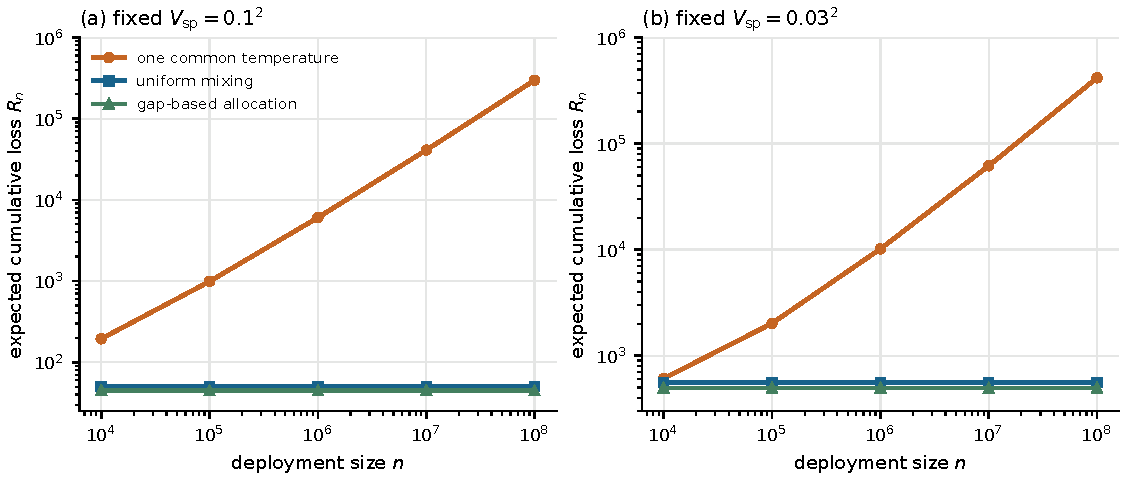
\includegraphics[width=0.92\textwidth]{figs/fig3_exploration_costs.pdf}
\caption{Exploration loss as deployment size increases, using the archived
deterministic calculations with $H\sim U(-1,1)$, $g(h)=|h|$, $\sigma^2=1$,
and fixed $V_{\rm sp}=\delta^2$. Curves share the same sparse-exploration
criterion, not verified equal finite-sample MSE. Context-dependent
temperature implements the gap-based probabilities and gives the same curve.
The panels have different vertical ranges.}
\label{fig:costs}
\end{figure}

\paragraph{Boundary inference.} Table~\ref{tab:boundary} reports the boundary
estimator of Theorem~\ref{thm:boundary}. Exploration loss matches the constant
in Theorem~\ref{thm:boundary}(v). With $\zeta=0.6$ coverage is close to
nominal; at $n=10^6$, 5,000 replications give \covFiveK{} (MCSE
\covFiveKmcse), with the estimated standard error at \covFiveKseRatio{} of the
Monte Carlo standard deviation. With a very small boundary sample the interval
under-covers: \covSmallNtau{} at $n\tau_n\approx\smallNtau$. The guarantee of
Theorem~\ref{thm:boundary} is asymptotic.

\paragraph{Temperature sweep.} Figure~\ref{fig:sweep} fixes $n=\curveN$ and
sharpens a common temperature, with \curveReps{} replications per temperature.
Wald coverage of the population effect falls from \curvePopCovLo{} at $1/\tau=1$
to \curvePopCovHi{} (Horvitz--Thompson) and \curveAipwCovHi{} (augmented
estimator) at $1/\tau=\curveInvTauMax$. Over the same range, coverage of the
boundary effect rises from \curveBndCovLo{} to \curveBndCovHi{}, and the
exploration loss falls from \curveLossLo{} to \curveLossHi{}. The Monte Carlo
error of the population estimators understates their exact standard deviation
once the policy is sharp: at $1/\tau=\curveInvTauMax$ the Monte Carlo root mean
squared error of the Horvitz--Thompson estimator is \curveHtMcRmseHi{}, while its
exact standard deviation is of order $10^{\curveHtExactSdHiExp}$. Its variance is
carried by rare, very large terms that the replications do not observe. For the
population estimators, the exact curves rather than the Monte Carlo points
describe the error.

\begin{figure}[htbp]
\centering
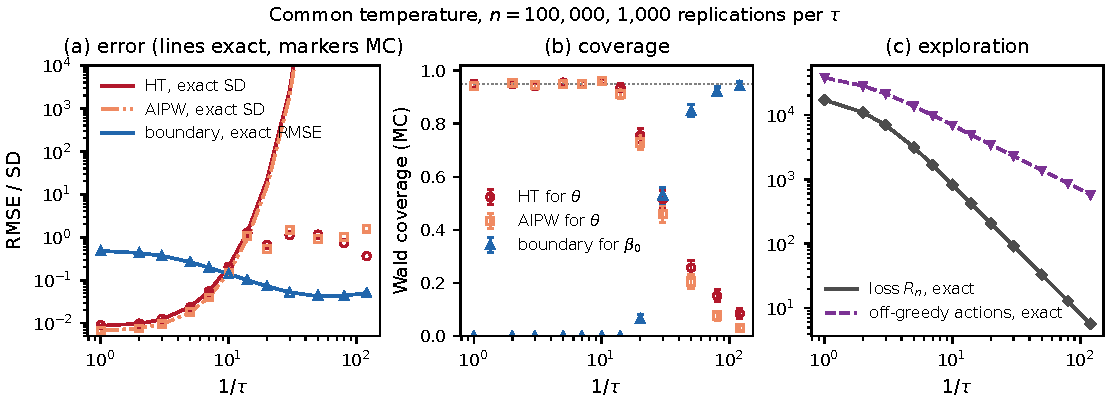
\includegraphics[width=\textwidth]{figs/fig4_temperature_sweep.pdf}
\caption{Common temperature at fixed $n=\curveN$, \curveReps{} replications
per temperature, same design as Figure~\ref{fig:map}. (a) Lines: exact standard
deviation of the Horvitz--Thompson and augmented (true regression) estimators
of $\theta$, and exact root mean squared error of the boundary estimator of
$\beta_0$. Markers: Monte Carlo root mean squared error; the augmented
estimator uses a linear working model. (b) Wald coverage with 95\% Monte Carlo
intervals. Boundary coverage is low while $n\tau^3$ is large, as
Theorem~\ref{thm:boundary}(iv) requires. (c) Exploration loss $R_n$ and expected
number of off-greedy actions; lines are exact, markers Monte Carlo.}
\label{fig:sweep}
\end{figure}

\begin{table}[htbp]
\centering\small
\tabBoundary
\caption{Boundary inference under common temperature $\tau_n=n^{-\zeta}$.
Coverage is of $\beta_0=c(0)$. Loss is the Monte Carlo mean with the
Theorem~\ref{thm:boundary}(v) constant in parentheses. The last row is a
separate 5,000-replication run.}
\label{tab:boundary}
\end{table}

%=============================================================================
\section{Discussion}\label{sec:discussion}

The results separate two uses of adaptive logs. If the question is how
outcomes respond where the deployed policy is indifferent, under the boundary assumptions, a growing deployment permits
increasingly precise local inference while cumulative exploration loss
vanishes. The number of exploratory actions still grows; their average
operational cost falls. If the question is the population average effect of a strategy,
uniformly consistent estimation over the model requires divergent
worst-case exploration loss. Increasing deployment size does not remove
that requirement. Reporting an effect estimated from adaptive logs therefore requires saying
which of the two quantities it is.

For design, the relevant choice is not whether to use temperature but how.
With one temperature shared by all contexts, the exploration probability
decays exponentially in the policy's confidence, so reaching confident
contexts forces a temperature that is costly near the boundary; uniform
mixing, context-dependent temperatures, or temperature mixtures with a
vanishing weight on a moderate temperature avoid this. Among designs that
avoid it, allocating by the value gap saves further loss when gaps are
heterogeneous and reasonably well specified (Lemma~\ref{lem:robust}); in our
example the saving is about ten percent.

\paragraph{Limitations.} The policy is known and assignments are logged; the
setting is a single decision per unit with independent contexts; the boundary
results are one-dimensional and pointwise; the population impossibility
excludes models in which boundary data identify the population effect; and
the treatment is strategy assignment under a fixed generator, not the realized
text. Extending the separation to multi-turn conversations requires defining
the reference policy for later turns and the induced distribution of histories,
which we leave open. Estimated policies, multidimensional scores and effects
of realized text features are also outside the formal results.


\section*{Data availability statement}
No new participant data were collected or analysed. The results are
theoretical, deterministic numerical illustrations, or simulations. The
simulation code, the result files (with arguments, random seeds and code
commits), plain-text versions of the proofs, and the scripts that generate
every number, table and figure in the paper are available in
the repository
\begin{center}\url{https://github.com/kunhailP/when-treatment-talks-back}\end{center}
(branch \texttt{jci-separation}, tagged submission version
\textbf{[TO CONFIRM: tag or commit]}).

\section*{Author contributions}
The author confirms sole responsibility for the conception of the study, the
theoretical results and proofs, the simulations, and the preparation of the
manuscript, and has approved the final version.

\section*{Conflict of interest}
\textbf{[TO CONFIRM]} The author states no conflict of interest.

\section*{Funding}
\textbf{[TO CONFIRM]} This research received no external funding.

\section*{Use of AI-assisted tools}
\textbf{[TO CONFIRM against the publisher's policy]} Generative AI tools were
used to assist in drafting text, checking proofs, and writing simulation code.
The author reviewed all content and takes full responsibility for it.

\begingroup\sloppy
\bibliographystyle{vancouver}
\bibliography{../references}
\endgroup

\appendix
% Proofs for main_jci.tex. Plain-text versions with the same content:
% theory/separation/{theorem_D,theorems_A_B_C,corollary_S}.md

\section{Proof of Theorem~\ref{thm:boundary}}\label{app:boundary}

Write $p=\sgm(H/\tau)$, $\omega=p(1-p)=K(H/\tau)$ with $K(u)=e^u/(1+e^u)^2$,
and $m_\tau=\E\omega$. We use
\[
\int K=1,\quad \int|u|K(u)\,du=2\log2,\quad \int K(u)\sgm(u)\,du=\tfrac12,\quad
K(u)\le e^{-|u|},\quad \int_0^\infty v\,\sgm(-v)\,dv=\tfrac{\pi^2}{12}.
\]

\paragraph{Step 1 (kernel integrals).} For $q$ bounded and continuous at $0$,
$j\ge1$ and $r,s\ge0$, substituting $h=\tau u$ and using dominated convergence
with dominating function $\|q\|_\infty\bar fK(u)$,
\[
\E[K(H/\tau)^j(1-p)^rp^sq(H)]=\tau f(0)q(0)\int K^j\sgm(-u)^r\sgm(u)^s\,du+o(\tau).
\]
In particular $m_\tau=\tau f(0)(1+o(1))$.

\paragraph{Step 2 (bias).} $\beta_{\ov,\tau}-\beta_0=\E[\omega\{c(H)-c(0)\}]/m_\tau$.
On $|H|\le u_0$, $|c(h)-c(0)|\le2L|h|$ and
$\E[\omega|H|]\le\bar f\tau^2\int|u|K=2\log2\,\bar f\tau^2$. On $|H|>u_0$,
$\omega\le e^{-u_0/\tau}$ and $|c(h)-c(0)|\le4B$. Hence
$|\beta_{\ov,\tau}-\beta_0|\le(4\log2\,L\bar f\tau^2+4Be^{-u_0/\tau})/m_\tau
=(4\log2\,L\bar f/f(0))\tau(1+o(1))$.

\paragraph{Step 3 (linearization).} Let $\bar\mu_a=\E[\omega\mu_a]/m_\tau$, so
$\bar\mu_1-\bar\mu_0=\beta_{\ov,\tau}$. Since $\E[w_1\mid H]=\omega$ and
$\E[w_1Y\mid H]=\omega\mu_1$, $\E[w_1(Y-\bar\mu_1)]=0$, and likewise for arm
$0$. Define $T_a=n^{-1}\sum_iw_{ai}(Y_i-\bar\mu_a)/m_\tau$ and
$\xi_i=\{w_{1i}(Y_i-\bar\mu_1)-w_{0i}(Y_i-\bar\mu_0)\}/m_\tau$. Then
$\hat m_a-\bar\mu_a=(m_\tau/\hat D_a)T_a$ and $\E\xi=0$. Because $w_1w_0=0$ and
$\E[A(1-p)^2\mid H]=\omega(1-p)$,
\[
s_n^2:=\Var\xi=m_\tau^{-2}\E\big[\omega\{(1-p)(\sigma_1^2+(\mu_1-\bar\mu_1)^2)+p(\sigma_0^2+(\mu_0-\bar\mu_0)^2)\}\big].
\]
By Step 1, $\bar\mu_a\to\mu_a(0)$; the terms in $(\mu_a-\bar\mu_a)^2$ are
$o(\tau)$ by dominated convergence; and the variance terms equal
$\tau f(0)\sigma_a^2(0)/2+o(\tau)$. Hence
$s_n^2=\{\sigma_1^2(0)+\sigma_0^2(0)\}/\{2\tau f(0)\}(1+o(1))$.

\paragraph{Step 4 (central limit theorem).} Since $0\le w_a\le1$, $w_a^4\le
w_a$, and $\E[(Y-\bar\mu_a)^4\mid A,H]\le C(M,B)$, we get
$\E[w_a^4(Y-\bar\mu_a)^4]\le Cm_\tau$ and $\E\xi^4\le C'm_\tau^{-3}$. The
Lyapunov ratio $n^{-1}\E\xi^4/s_n^4\asymp(n\tau)^{-1}\to0$, so
$n^{-1/2}\sum\xi_i/s_n\Rightarrow N(0,1)$. Also
$\Var(\hat D_a)/m_\tau^2\le1/(nm_\tau)\to0$, so $\hat D_a/m_\tau\to1$ in
probability and $m_\tau/\hat D_a-1=O_p((n\tau)^{-1/2})$. Now
\[
\hat\beta-\beta_{\ov,\tau}=(T_1-T_0)+(m_\tau/\hat D_1-1)T_1-(m_\tau/\hat D_0-1)T_0,
\]
with $T_1-T_0=n^{-1}\sum\xi_i$ and $T_a=O_p((n\tau)^{-1/2})$. The remainder is
$O_p((n\tau)^{-1})=o_p(s_n/\sqrt n)$, and Slutsky's lemma gives (i).

\paragraph{Step 5 (variance estimator).} Write
$\xi_{ai}=w_{ai}(Y_i-\bar\mu_a)/m_\tau$. First, $n^{-1}\sum\xi_i^2/s_n^2$ has
mean one and variance at most $\E\xi^4/(ns_n^4)\asymp(n\tau)^{-1}$. Second,
\[
\hat\psi_{1i}-\xi_{1i}=w_{1i}(Y_i-\bar\mu_1)(1/\hat D_1-1/m_\tau)+w_{1i}(\bar\mu_1-\hat m_1)/\hat D_1 .
\]
The mean square of the first term is
$(n^{-1}\sum\xi_{1i}^2)(m_\tau/\hat D_1-1)^2=O_p(s_n^2)O_p((n\tau)^{-1})$.
For the second, $w_1^2\le w_1$ gives mean square at most
$(\hat m_1-\bar\mu_1)^2/\hat D_1$; by Step 4 and $\hat D_1=\tau f(0)(1+o_p(1))$
this is $O_p(1/(n\tau^2))$, which is $O_p((n\tau)^{-1})$ relative to
$s_n^2\asymp\tau^{-1}$. Arm $0$ is identical. By Minkowski's and the
Cauchy--Schwarz inequalities, $|n^{-1}\sum\hat\psi_i^2-n^{-1}\sum\xi_i^2|=o_p(s_n^2)$,
which gives (iii).

\paragraph{Step 6 (centering at $\beta_0$).}
$(\beta_{\ov,\tau}-\beta_0)/(s_n/\sqrt n)=O(\tau)O((n\tau)^{1/2})=O((n\tau^3)^{1/2})$.
With (i), (iii) and Slutsky's lemma this gives (iv).

\paragraph{Step 7 (exploration loss).} The off-greedy probability is
$\sgm(-|h|/\tau)$. On $|h|\le u_0$,
$n\E[\phi(|H|)\sgm(-|H|/\tau)]\le n\bar\kappa\bar f\cdot2\tau^2\int_0^\infty
v\sgm(-v)dv=n\bar\kappa\bar f\tau^2\pi^2/6$, and the rest is at most
$n\bar Ge^{-u_0/\tau}$. In the strong form, on $v\le u_0/\tau$,
$\phi(\tau v)/\tau\to\kappa v$ and $f(\tau v)\to f(0)$ with dominating function
$\bar\kappa v\bar f\sgm(-v)$, which gives the asymptotic equality. For
$\tau_n=n^{-\zeta}$: $n\tau_n\to\infty$ iff $\zeta<1$; $n\tau_n^3\to0$ iff
$\zeta>1/3$; $n\tau_n^2\to0$ iff $\zeta>1/2$. \qed

\paragraph{Smoother effects.} If $|c(h)-c(0)-c'(0)h|\le M_2h^2$ and $f$ is
$L_f$-Lipschitz near $0$, then
$\E[\omega H]=\tau^2\int uK(u)\{f(\tau u)-f(0)\}du=O(\tau^3)$ up to an
exponentially small tail, and the quadratic remainder contributes at most
$M_2\bar f\tau^3\int u^2K/m_\tau$; the bias is $O(\tau^2)$. Differentiability of
$c$ alone is not enough: $c(h)=1+|h|^{3/2}$ gives bias
$\tau^{3/2}\int|u|^{3/2}K(u)du\,(1+o(1))$.

%-----------------------------------------------------------------------------
\section{Proofs for Section~\ref{sec:population}}\label{app:population}

\paragraph{Proof of Theorem~\ref{thm:info}.}
\emph{Submodel.} For $\vartheta\in[-B,B]^K$ set $\mu^\vartheta_{a^*(h)}(h)=0$,
and on $S_k$ set $\mu^\vartheta_{\bar a(h)}(h)=s_k\vartheta_k$ with $s_k=+1$ if
$\bar a=1$ on $S_k$ and $s_k=-1$ otherwise; elsewhere
$\mu^\vartheta_{\bar a(h)}(h)=0$. Then $\mu^\vartheta\in\M(B,\sigma)$ and
$\theta(\mu^\vartheta)=\sum_kf_k\vartheta_k$.

\emph{Information.} The sample density is
$\prod_idF(H_i)\,\kappa_i(A_i\mid H_i,\mathcal F_{i-1})\,\varphi_\sigma(Y_i-\mu^\vartheta_{A_i}(H_i))$,
where the assignment kernels $\kappa_i$ are known functions of observed data.
The score for $\vartheta_k$ is
$\sum_i\mathbf 1\{H_i\in S_k,A_i=\bar a(H_i)\}s_k(Y_i-s_k\vartheta_k)/\sigma^2$.
Its summands are martingale differences, so the Fisher information matrix is
diagonal with $I_k(\vartheta)=\E_\vartheta N_k/\sigma^2$, where
$N_k=\sum_i\mathbf 1\{H_i\in S_k,A_i=\bar a(H_i)\}$.

\emph{van Trees.} Take the product prior with marginal density
$B^{-1}\cos^2(\pi x/(2B))$ on $[-B,B]$, whose Fisher information is $J=\pi^2/B^2$.
With $\bar N_k=\int\E_\vartheta N_k\,\lambda(d\vartheta)$, the multivariate van
Trees inequality \citep{gill1995applications}, maximized over the direction
vector, gives
\[
\sup_{\M(B,\sigma)}\E(\hat\theta-\theta)^2\ge\sum_k\frac{f_k^2}{\bar N_k/\sigma^2+J}=\sum_k\frac{f_k\sigma^2}{a_k},
\qquad a_k=\frac{\bar N_k+\sigma^2J}{f_k}.
\]

\emph{Cauchy--Schwarz and loss.} Writing
$\sigma\sum_kf_k\sqrt{g_k}=\sum_k\sqrt{f_kg_ka_k}\cdot\sigma\sqrt{f_k/a_k}$,
\[
\sigma^2\Big(\sum_kf_k\sqrt{g_k}\Big)^2\le\Big(\sum_kf_kg_ka_k\Big)\Big(\sum_kf_k\sigma^2/a_k\Big).
\]
Here $\sum_kf_kg_ka_k=\sum_kg_k\bar N_k+\sigma^2J\sum_kg_k$, and since $g\ge g_k$
on $S_k$, $\sum_kg_kN_k\le\sum_ig(H_i)\mathbf 1\{A_i=\bar a(H_i)\}$, so
$\sum_kg_k\bar N_k\le\sup R_n$. This proves \eqref{eq:info}.

\emph{Consequences.} With $K=1$ and $S_1=\{g\ge\gamma\}\cap\{a^*=j\}$ of positive
mass, \eqref{eq:info} gives
$\sup R_n\ge g_1\{\sigma^2f_1^2/\sup\E(\hat\theta-\theta)^2-\sigma^2\pi^2/B^2\}\to\infty$.
For the constant, fix a partition into level sets of $g$ intersected with the
two greedy sides; \eqref{eq:info} gives
$\liminf\delta_n^2\sup R_n\ge\sigma^2(\sum f_k\sqrt{g_k})^2$, and lower sums
$\sum F(S)\inf_S\sqrt g$ increase to $\E\sqrt g$ as the level mesh shrinks. \qed

\paragraph{Proof of Proposition~\ref{prop:achieve}.} The Horvitz--Thompson
estimator is unbiased with variance at most
$n^{-1}(\sigma^2+B^2)\E[1/e_1+1/(1-e_1)]\le n^{-1}(\sigma^2+B^2)(\E[1/p]+2)$,
where $e_1=\Prob(A=1\mid H)$. Pointwise $1/p=\max\{2,\sqrt g/c_n\}\le\sqrt g/c_n+2$,
and the choice of $c_n$ gives $\E[1/p]+2\le n\delta_n^2/(\sigma^2+B^2)$. The
loss is $n\E[gp]\le nc_n\E\sqrt g$. The uniform design is analogous. \qed

%-----------------------------------------------------------------------------
\section{Proof of Theorem~\ref{thm:separation}}\label{app:separation}

The function $b$ satisfies $0\le b\le1$, is $\pi/(u_2-u_1)$-Lipschitz, vanishes on
$(-\infty,u_1]$, and has $\E b(H)>0$ because $H$ has a density and
$F([u_1,u_2])>0$. Hence $|tb|\le B$ and $tb$ is $L$-Lipschitz for
$|t|\le t_{\max}$, so $\mu^t\in\M_D$; $c^t=tb$, $\beta_0(\mu^t)=0$, and
$\theta(\mu^t)=t\E b(H)$. Every perturbed observation is off-greedy, since
$a^*=1$ on $(0,\infty)$, with $H\in[u_1,u_2]$. Let
$N=\sum_i\mathbf 1\{A_i=0,H_i\in[u_1,u_2]\}$.

\emph{(S1)} is Theorem~\ref{thm:boundary}, because every member of $\M_D$
satisfies Assumption~\ref{ass:D}.

\emph{(S2).} The sample densities under $\mu^0$ and $\mu^t$ coincide on
$E=\{N=0\}$, so $P_0(E)=P_t(E)$, and for any event $A$,
$|P_0(A)-P_t(A)|=|P_0(A\cap E^c)-P_t(A\cap E^c)|\le\max\{P_0(E^c),P_t(E^c)\}=P_0(E^c)$.
Thus $\TV\le P_0(N\ge1)\le\E_0N$. Because $g\ge\gamma$ $F$-almost surely on
$[u_1,u_2]$ and $H_i\sim F$, $\gamma N\le\sum_ig(H_i)\mathbf 1\{A_i=\bar a(H_i)\}$
almost surely, so $\E_0N\le R_n(\mu^0)/\gamma$. Le Cam's two-point argument with
separation $t_1\E b$ gives the displayed bound.

\emph{(S3).} The score of $t\mapsto\mu^t$ is
$\sum_i\mathbf 1\{A_i=0\}(-b(H_i))(Y_i+tb(H_i))/\sigma^2$, with information
$I(t)=\E_t\sum_i\mathbf 1\{A_i=0\}b(H_i)^2/\sigma^2\le\E_tN/\sigma^2\le R_n(\mu^t)/(\gamma\sigma^2)$.
With the prior $t_{\max}^{-1}\cos^2(\pi t/(2t_{\max}))$ on $[-t_{\max},t_{\max}]$,
whose information is $\pi^2/t_{\max}^2$, the van Trees inequality for
$\psi(t)=t\E b$ gives the bound. \qed

%-----------------------------------------------------------------------------
\section{Proofs for Section~\ref{sec:temperature}}\label{app:temperature}

\paragraph{Proof of Theorem~\ref{thm:common}.} Take the single cell
$S=\{|\Delta|\ge G-\eta',a^*=j\}$, with $j$ attaining $q=q_{\eta'}$. There
$p\le e^{-(G-\eta')/\tau}$, so $\bar N\le nqe^{-(G-\eta')/\tau}$, and the van
Trees step of Theorem~\ref{thm:info} with $K=1$ gives
$\delta_n^2\ge q^2\sigma^2/(nqe^{-(G-\eta')/\tau}+\sigma^2\pi^2/B^2)$. Once
$\delta_n^2\le q^2B^2/(2\pi^2)$, this forces
$nqe^{-(G-\eta')/\tau}\ge q^2\sigma^2/(2\delta_n^2)$, that is,
$\tau_n\ge(G-\eta')/\log\{2n\delta_n^2/(q\sigma^2)\}$. On the other hand
$R_n=n\E[\phi(|\Delta|)\sgm(-|\Delta|/\tau)]\ge n\kappa f_{\min}\tau^2\int_0^{u_0/\tau}v\sgm(-v)dv\ge
n\kappa f_{\min}c_0\min\{\tau,u_0\}^2$. Combining the two displays proves the
claim. With finitely many score values, the same argument gives
$\tau\ge\Delta_{\max}/\log(Cn\delta^2)$ for $\delta$ small enough, and the
$\Delta_{\min}$ cell contributes $n f\phi(\Delta_{\min})e^{-\Delta_{\min}/\tau}/2$. \qed

\paragraph{Remark~\ref{rem:mixture}.} With $q=\sgm(-u)$ and
$p_n=w_nq+(1-w_n)\sgm(-nu)$, $p_n\ge w_nq$ gives $\E[1/p_n]/n\le\delta^2$ for
$w_n=\E[1/q]/(n\delta^2)$, and $n\E[up_n]\le\E[1/q]\E[uq]/\delta^2+O(1/n)$. With
$w_n=\E[1/q]/\{n\delta_n^2/(\sigma^2+B^2)-2\}$ the Horvitz--Thompson risk is at
most $\delta_n^2$ uniformly over $\M(B,\sigma)$.

\paragraph{Proof of Proposition~\ref{prop:ctx}.} Solving
$\sgm(-|\Delta|/\tau)=p$ gives the formula. For $p^*=c_n/\sqrt{\phi(|\Delta|)}<1/2$,
$\log\{(1-p^*)/p^*\}=\log(1/c_n)+\tfrac12\log\phi(|\Delta|)+\log(1-p^*)$, and
$c_n\to0$. On $\{\Delta=0\}$, $g=\phi(0)=0$, so $p^*=1/2$. \qed

\paragraph{Proof of Lemma~\ref{lem:robust}.} With $p=c/\sqrt{\hat g}$ and
$\E[1/p]=T$, the loss is $n\E[\sqrt{\hat g}]\E[g/\sqrt{\hat g}]/T$, against
$n(\E\sqrt g)^2/T$ for $\hat g=g$. With $s=(\hat g/g)^{1/2}\in[\sqrt a,\sqrt b]$
and the probability measure $w\propto\sqrt g\,dF$, the ratio is
$\E_w[s]\E_w[1/s]$, which Kantorovich's inequality bounds by
$(\sqrt a+\sqrt b)^2/(4\sqrt{ab})=K(b/a)$. If $w$ has a set of mass one half,
setting $s=\sqrt a$ there and $s=\sqrt b$ elsewhere attains the bound. With
atoms the bound need not be attained: for $F=(0.99,0.01)$, $g=(1,100)$ and
$\rho=36$, uniform mixing costs $1.675$ times the optimum, below $K(36)=2.042$,
yet every admissible $\hat g$ costs at most $1.347$ times the optimum. \qed


\end{document}

